\documentclass{article}
\usepackage{tikz}
\usepackage{caption}
\begin{document}
\begin{center}
\Large{\textbf{Hierarchy of Linux Distributions}}
\end{center}
\vspace{1cm}
\begin{figure}[h]
\centering
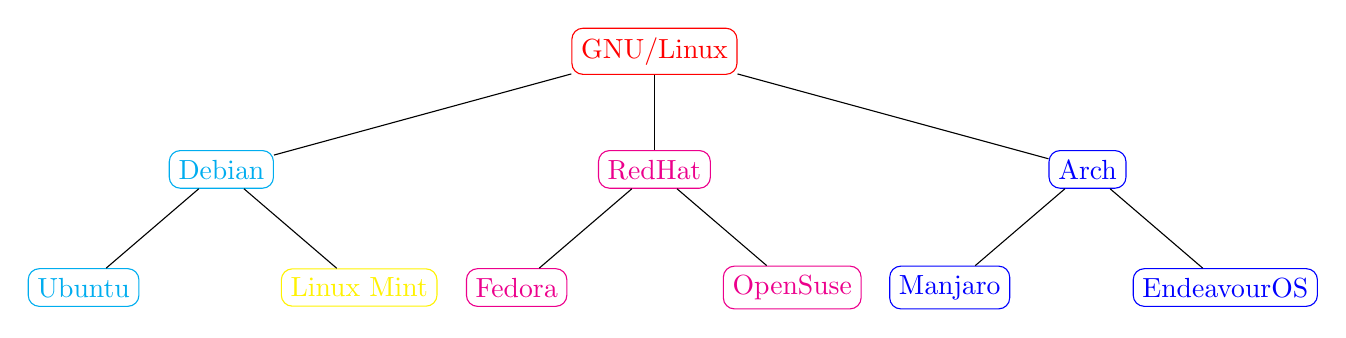
\begin{tikzpicture}[
every node/.style={draw, rounded corners},
level 1/.style={sibling distance=55mm},
level 2/.style={sibling distance=35mm}
]

\node[red] {GNU/Linux}
    child {node[cyan] {Debian}
        child {node[cyan] {Ubuntu}}
        child {node[yellow] {Linux Mint}}
    }
    child {node[magenta] {RedHat}
        child {node[magenta] {Fedora}}
        child {node[magenta] {OpenSuse}}
    }
    child {node[blue] {Arch}
        child {node[blue] {Manjaro}}
        child {node[blue] {EndeavourOS}}
    };
\end{tikzpicture}
\vspace{1cm}
\caption*{GNU/Linux Operating System Family}


\end{figure}

\pagebreak

\begin{center}
\Large{\textbf{SUV Cars}}
\end{center}

\begin{figure}[h]
\centering
\begin{tikzpicture}[
grow=-45,
every node/.style={draw, rounded corners},
level 1/.style={sibling distance=65mm},
level 2/.style={sibling distance=45mm}
]

\node[red] {SUV}
    child {
        node[cyan] {Tata}
        child {node[cyan] {Nexon}}
        child {node[cyan] {Punch}}
    }
    child {
        node[magenta] {Volkswagen}
        child {node[magenta] {Taigun}}
        child {node[magenta] {Virtus}}
    }
    child {
        node[blue] {Maruti}
        child {node[blue] {Brezza}}
        child {node[blue] {Vitara}}
    };

\end{tikzpicture}
\caption*{Car Brands Hierarchy}

\end{figure}

\end{document}